\documentclass[10pt,a4paper]{article}
\usepackage[utf8]{inputenc}
\usepackage[T1]{fontenc}
\usepackage{amsmath}
\usepackage{amssymb}
\usepackage{graphicx}
\usepackage{multicol, multirow}
\usepackage{booktabs}
\usepackage{rotating}
\usepackage{setspace}
\graphicspath{{images/}}
\title{Data Mining; Assignemt 4}
\author{Jesse Annan \hspace{0.5cm} | \hspace{0.5cm} ID: 002708111}
\newcommand{\h}{\textbf{H}}
\newcommand{\ig}{\textbf{InfoGain}}
%\newcommand{\hsyg}{\h(sprinkler = yes | grass)}
\newcommand{\sdw}{\displaystyle{ \sum_{i \in \{dry, wet\}} }}
\newcommand{\x}{\mathbb{X}}
\newcommand{\cc}{\mathbb{C}}
\newcommand{\p}{\textbf{P}}
\begin{document}
	\maketitle

    \clearpage
 
	\begin{enumerate}
		\item \textbf{Question 1} \newline
		First we need to determine the root node - the feature with most information gain. \newline
		This is obtained by calculating the weighted entropy of each attribute and taking it out of the entropy of the datasets (Grass). \newline
			\textbf{Step 1: Determining Root Node:} \newline
				\begin{equation*}
						\begin{split}
							\h(grass) & = - \sdw p(i) \cdot \log_2 p(i) \\
							& = - ( (9/16)\times\log_2(9/16) + (7/16)\times\log_2(7/16) ) = .9887
						\end{split}
				\end{equation*}
			
				\begin{equation*}
					\begin{split}
						\h(sprinkler=yes | grass) & = \sdw p(i) \cdot \log_2 p(i) \\
						& = -( (1/6)\times\log_2(1/6) + (5/6)\times\log_2(5/6) ) = .6500 \\
						\h(sprinkler=no | grass) & = \sdw p(i) \cdot \log_2 p(i \\
						& = -( (8/10)\times\log_2(8/10) + (2/10)\times\log_2(2/10) ) = .7219 \\
						\ig(Sprinkler) & = \frac{\# \textit{sprinkler=yes}}{n} \times \h(sprinkler=yes | grass) \\
						& + \frac{\# \textit{sprinkler=no}}{n} \times \h(sprinkler=no | grass) \\
						& = \frac{6}{16} \times .6500 + \frac{10}{16} \times .7219 = .2937
					\end{split}
				\end{equation*}
			
				\begin{equation*}
					\begin{split}
						\h(rain=yes | grass) & = \sdw p(i) \cdot \log_2 p(i) \\
						& = -( (1/4)\times\log_2(1/4) + (3/4)\times\log_2(3/4) ) = .8113 \\
						\h(rain=no | grass) & = \sdw p(i) \cdot \log_2 p(i \\
						& = -( (8/12)\times\log_2(8/12) + (4/12)\times\log_2(4/12) ) = .9183 \\
						\ig(rain) & = \frac{\# \textit{rain=yes}}{n} \times \h(rain=yes | grass) \\
						& + \frac{\# \textit{rain=no}}{n} \times \h(rain=no | grass) \\
						& = \frac{4}{16} \times .8113 + \frac{12}{16} \times .9183 = .0972
					\end{split}
				\end{equation*}
		
		Since \ig(sprinkler) is greater than the \ig(rain), we select sprinkler as our parent node.
		\begin{figure}[h!]
			\centering
			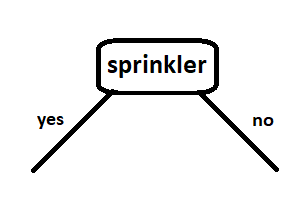
\includegraphics[scale=.5]{pnode}
		\end{figure}
		
		\textbf{Step 2: Determining Sub Root Node:} \newline
		Now, we determine the sub root for our parent root i.e given sprinkler what is the information gain
		
%			\item \begin{equation*}
%				\begin{split}
%					\h(grass | sprinkler = no) & = - \sdw p(i) \cdot \log_2 p(i) \\
%					& = - ( (8/10)\times\log_2(8/10) + (2/10)\times\log_2(2/10) ) = .7219
%				\end{split}
%			\end{equation*}
			
			\begin{equation*}
				\begin{split}
					\h(rain=yes | grass, sprinkler = no) & = \sdw p(i) \cdot \log_2 p(i) \\
					& = -( (1/3)\times\log_2(1/3) + (2/3)\times\log_2(2/3) ) = .9183 \\
					\h(rain=no | grass, sprinkler = no) & = \sdw p(i) \cdot \log_2 p(i \\
					& = - (7/7)\times\log_2(7/7) = 0 \\
%					\ig(rain | sprinkler = no) & = \frac{\# \textit{sprinkler=yes}}{n} \times \h(sprinkler=yes | grass) \\
%					& + \frac{\# \textit{sprinkler=no}}{n} \times \h(sprinkler=no | grass) \\
%					& = \frac{6}{16} \times .6500 + \frac{10}{16} \times .7219 = .2937
				\end{split}
			\end{equation*}
		
%			\item \begin{equation*}
%				\begin{split}
%					\h(grass | sprinkler = yes) & = - \sdw p(i) \cdot \log_2 p(i) \\
%					& = - ( (1/6)\times\log_2(1/6) + (5/6)\times\log_2(5/6) ) = .6500
%				\end{split}
%			\end{equation*}
			
			\begin{equation*}
				\begin{split}
					\h(rain=yes | grass, sprinkler = yes) & = \sdw p(i) \cdot \log_2 p(i) \\
					& = (1/1)\times\log_2(1/1) = 0 \\
					\h(rain=no | grass, sprinkler = yes) & = \sdw p(i) \cdot \log_2 p(i) \\
					& = -( (1/5)\times\log_2(1/5) + (4/5)\times\log_2(4/5) ) = .7219 \\
%					\ig(rain) & = \frac{\# \textit{rain=yes}}{n} \times \h(rain=yes | grass) \\
%					& + \frac{\# \textit{rain=no}}{n} \times \h(rain=no | grass) \\
%					& = \frac{4}{16} \times .8113 + \frac{12}{16} \times .9183 = .0972
				\end{split}
			\end{equation*}
			
		Whenever we find \h \; = 0, it implies that there is one distinct class in the particular sample. Therefore, from our calculations, $\h(rain=yes | grass, sprinkler = yes) = 0$ means that whenever the sprinkler is on and it rains then the grass is wet similarly $ \h(rain=no | grass, sprinkler = no) = 0 $ means that whenever the sprinkler is off and it isn't raining then the grass is dry. 
		
		\begin{figure}[ht!]
			\centering
			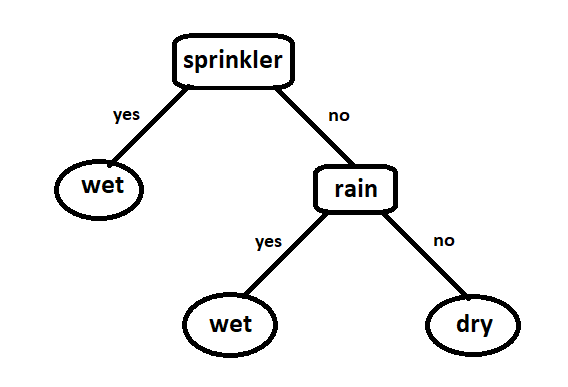
\includegraphics[scale=.5]{dtree}
		\end{figure}
		
		Also with the calculations we can conclude that there's $ 4/5 $ chance that the grass is wet if sprinkler is off and it's raining and also there's $ 2/3 $ chance that the grass is wet if the sprinkler is on and it's raining. Hence the decision tree above is the best three that David can obtain using information gain on \textbf{Table 1}.
		
		
		\clearpage
		\item \textbf{Question 2} \newline
			\begin{table}[h!]
				\centering
				\begin{tabular}{l|cccccccccc}
					\textbf{Actual} & Wet & Dry & Dry & Wet & Wet & Dry & Dry & Wet & Wet & Dry \\ \hline
					\textbf{Predicted} & Dry & Dry & Wet & Wet & Wet & Wet & Dry & Wet & Wet & Dry 
				\end{tabular}
			\end{table}
		
		\begingroup
		\renewcommand{\arraystretch}{1.5}
			\begin{table}[h!]
				\centering
				\begin{tabular}{c|c|c|c|c|}
					\multicolumn{5}{c}{\textbf{Confusion Matrix}} \\ \toprule
					\multicolumn{1}{c}{ \multirow{6}{*}{\rotatebox{90}{\textbf{Actual}}} } & \multicolumn{1}{c}{} & \multicolumn{2}{c}{\textbf{Predicted}} & \multicolumn{1}{c}{} \\ \cline{3-5}
					\multicolumn{1}{c}{} & & \textbf{Wet} & \textbf{dry} & \textbf{Total} \\ \cline{2-5}
					& \textbf{Wet} & 4 & 1 & 5 \\ 
					& \textbf{Dry} & 2 & 3 & 5 \\ \cline{2-5}
					& \textbf{Total} & 6 & 4 & 10 \\ \cline{2-5}
				\end{tabular}
			\end{table}
		
			\begin{table}[h!]
				\centering
				\begin{tabular}{l|l}
					\multicolumn{2}{c}{Accuracy Values} \\ \toprule
					Classification Accuracy & $\frac{4 + 3}{10} = .7 $ \\
					Error rate & $\frac{2 + 1}{10} = .3 $ \\
					Sensitivity & $\frac{4}{5} = .8 $ \\
					Precision & $\frac{4}{6} = .6667 $ \\
					Recall & $\frac{4}{5} = .8 $ \\
					F-score & $\frac{2 \times \frac{4}{6} \times \frac{4}{5} }{\frac{4}{6} + \frac{4}{5} } = .7273 $ \\ \bottomrule
				\end{tabular}
			\end{table}
		\endgroup
		
		
		\clearpage
		\item \textbf{Question 3} \newline
			Given $\x \; = \{ Rain = No, Sprinkler = Yes \}$ we want to find \newline
			$\textit{max } \p(\cc_i | \x_j) \hspace*{.2cm} \alpha \hspace*{.2cm} \p(\x_j | \cc_i) \cdot \p(\cc_i) $ \newline
			$ \Rightarrow \p(grass | \x_j) \hspace*{.2cm} \alpha \hspace*{.2cm} \p(\x_j | grass) \cdot \p(grass) $ \newline
			
			\begin{equation*}
				\begin{split}
					\p(grass = wet) & = \frac{7}{16} \\
					\p(grass = dry) & = \frac{9}{16} \\
					\p(rain = no | grass = wet) & = \frac{4}{7} \\
					\p(rain = no | grass = dry) & = \frac{8}{9} \\
					\p(sprinkler = yes | grass = wet) & = \frac{5}{7} \\
					\p(sprinkler = yes | grass = dry) & = \frac{1}{7} \\
					\p(\x | grass = wet) & = \p(rain = no | grass = wet) \\ & \times \p(sprinkler = yes | grass = wet) = \frac{20}{49} \\
					\p(\x | grass = dry) & = \p(rain = no | grass = dry) \\ & \times \p(sprinkler = yes | grass = dry) = \frac{8}{81} \\
					\p(grass = wet | \x) & = \p(\x | grass = wet) \times \p(grass = wet) = \frac{5}{28} \\
					\p(grass = dry | \x) & = \p(\x | grass = dry) \times \p(grass = dry) = \frac{1}{18}
				\end{split}
			\end{equation*}
		
			Since the value of $\p(grass = wet | \x) > \p(grass = dry | \x)$ our Na$\text{\"i}$ve Bayesian classifier will predict \newline \textbf{Grass = wet} for $\x \; = \{ Rain = No, Sprinkler = Yes \}$
		
		
		\clearpage
		\item \textbf{Question 4} \newline
		
		\begingroup
			\renewcommand{\arraystretch}{1.5}
			\begin{table}[h!]
				\centering
				\begin{tabular}{|c|c|}
					\multicolumn{2}{c}{\textbf{\p(Rain)}} \\ \toprule
					\textbf{no} & $\frac{12}{16}$ \\
					\textbf{yes} & $\frac{4}{16}$ \\ \hline
				\end{tabular}
			\end{table}
		
			\begin{table}[h!]
				\centering
				\begin{tabular}{c|c|c|c|}
					\multicolumn{4}{c}{\textbf{\p(Sprinkler | Rain)}} \\ \toprule 
					\multicolumn{2}{c}{ } & \multicolumn{2}{c}{ \textbf{Sprinkler} } \\ \cline{3-4}
					\multicolumn{1}{c}{ \multirow{4}{*}{ \rotatebox{90}{\textbf{Rain}} }} & & \textbf{no} & \textbf{yes} \\ \cline{2-4}
					& \textbf{no} & $\frac{7}{12}$ & $\frac{5}{12}$ \\
					& \textbf{yes} & $\frac{3}{4}$ & $\frac{1}{4}$ \\ \cline{2-4}
				\end{tabular}
			\end{table}
		
			\begin{table}[h!]
				\centering
				\begin{tabular}{|c|c|c|c|}
					\multicolumn{4}{c}{\textbf{\p(Grass |Rain, Sprinkler)}} \\ \toprule 
					\multicolumn{2}{c}{ } & \multicolumn{2}{c}{ \textbf{Grass} } \\ \hline
					\textbf{Rain} & \textbf{Sprinkler} & \textbf{Wet} & \textbf{Dry} \\ \hline
					\textbf{No} & \textbf{No} & 0 & 1 \\
					\textbf{No} & \textbf{Yes} & $\frac{4}{5}$ & $\frac{1}{5}$ \\
					\textbf{Yes} & \textbf{No} & $\frac{2}{3}$ & $\frac{1}{3}$ \\
					\textbf{Yes} & \textbf{Yes} & 1 & 0 \\ \hline
				\end{tabular}
			\end{table}
		
		\endgroup
		
		\begin{figure}[h!]
			\centering
			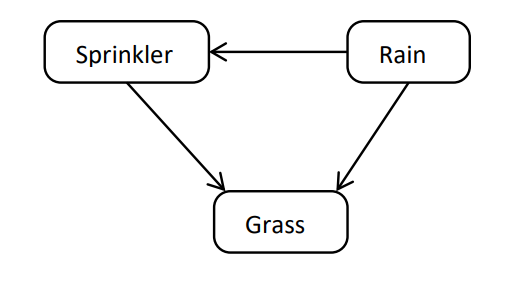
\includegraphics{nb}
		\end{figure}
		
	\end{enumerate}
	
\end{document}